\chapter{Results}
\label{sec:results}

In the following, the results of the thesis will be discussed.
The performance of the optimization routine will be shown for different settings, i.e. for different number of relays, receiving antennas per user, users, relay placings, ...
If not any further mentioned, the same settings will be used, as in Section~\ref{sec:solver}, i.e.
we will look at a 2x2 MIMO system with one receive antenna per user and three relays, as shown in Figure~\ref{fig:antenna_placing}.
The relays in this system will be lossless, i.e. the impedances will be pure imaginary.

\section{Introduction of Measures for Comparison}
\label{sec:measures}
To be able to rate the results, on how good they are, the performance will be compared to TDMA.
Additionally theoretical performance limits will be shown, in order to see by how much the performance could be pushed at maximum.

\subsection{Uncoupled Relay Rates}
One of the logical performances to compare the use of loaded antennas to, is the same setting without any coupling among the relays.
Logically, the "uncoupled relays rate" should be smaller than including and adapting the coupling to our needs.
If no higher rate can be achieved, the whole idea of using passive relays would fail.
\begin{figure}[h]
\centering
  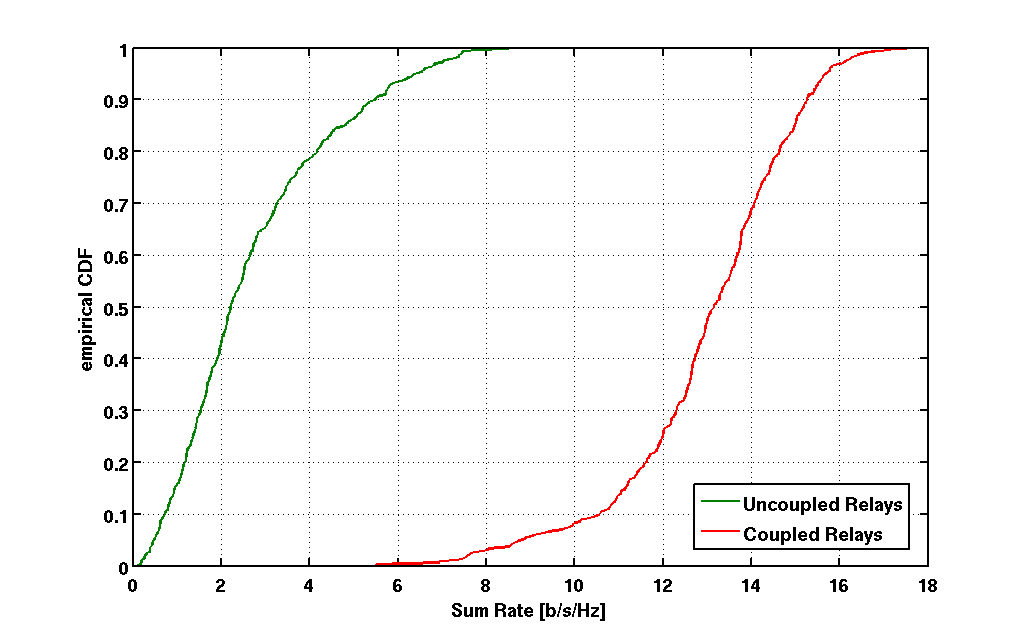
\includegraphics[width=0.7\linewidth]{images/Coupledcomparison.png}
\caption{Comparison of uncoupled relays and optimized coupled relays.}
\label{fig:coupledcomparison}
\end{figure}

In Figure~\ref{fig:coupledcomparison}, the green solid line shows the performance if no coupling among the relays and receivers exist.
It is clear, that the rates including relay coupling (red solid line) are much larger than without any coupling.

\subsection{TDMA Rates}
The next performance, the optimized rates are compared to are the TDMA rates for the equivalent setup.
Therefore, the relays are again assumed to be uncoupled from the receivers and the transmit/receive pairs are assumed to divide the time equally among each other for transmission.

FORMULAS (PRELOG-FACTOR)

\begin{figure}[h]
\centering
  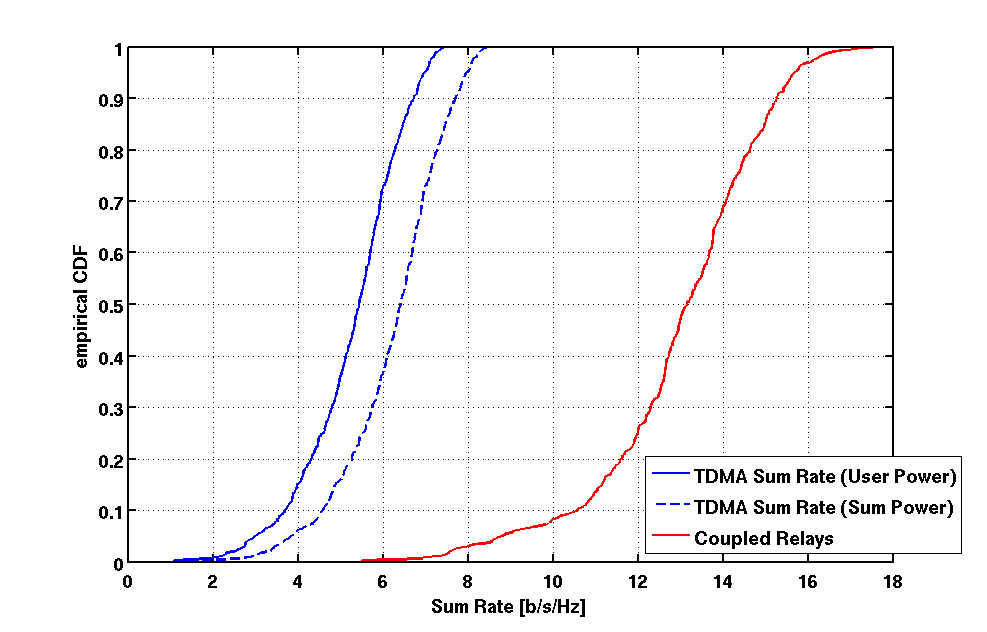
\includegraphics[width=0.7\linewidth]{images/TDMAcomparison.png}
\caption{Comparison of the TDMA rate and optimized coupled relays.}
\label{fig:TDMAcomparison}
\end{figure}

In Figure~\ref{fig:TDMAcomparison}, the blue solid line shows the performance if TDMA was applied under the user-power constraint (i.e. the limit of the transmit power is given per user and therefore the same for each user as in the coupled relay case) and the relays were uncoupled from the receivers.
The blue dashed line shows the performance of TDMA under the sum power constraint (i.e. the limit of the transmit power is given by the total transmit power and therefore the power per user in TDMA is $N_\text{User}$ times the power per user in the coupled relay case - here two times).
As before, the rates including relay coupling (red solid line) are much larger than without any coupling and TDMA.
Of course this comparison is more dependent on the choice of the settings (especially the choice of the number of transmit-receive pairs) and we will see different behaviors in the following sections. 

\subsection{Signal-Interference-Ration (SIR) Rates}
\label{sec:sir}
As we are addressing the problem of interference, a good measure is the SIR-rate.
It is calculated similar to the SINR-rate\eqref{eq:sinr_rate}, however it only considers the interference and not the noise.
As we said, in high SNR regime, the interference is the main diminishing factor for the rates (c.f. Section~\ref{sec:rates}), the SIR-rates will give us a indicator, on how good we optimized the relays.
Example curves of the SIR-rates (blue dashed lines) can be seen in Figures~\ref{fig:relcomp_1}~to~\ref{fig:relcomp_3}.

\subsection{Relays as Fully Cooperation Receivers - Limit}
\label{sec:fullrx_limit}
The remaining two function to which the optimization algorithms are compared against will give limits on how good the method of loaded antennas can be at best.
The first approach is to see the relays as fully cooperation receivers.
Therefore the number of observations the receiver has on the incoming signals is increased to $N_\text{Rx} + N_\text{Relays}$.
As we choose the number of relays always strictly larger than the number of interferer, this method will always lead to zero interference.

The performance of the fully cooperation relays can be seen in Figure~\ref{fig:limcomparison} (black solid curve).
At median it is almost $2 \left[\text{b/s/Hz}\right]$ higher, than the optimized rate of the passive coupled relays.
For the best 10\% of the cases this is reduced to $1 \left[\text{b/s/Hz}\right]$ and less,
for the worst 10\% of the cases this lies in between  $2.5 \left[\text{b/s/Hz}\right]$ and $4.7 \left[\text{b/s/Hz}\right]$.


\subsection{Multiport Matching - Limit}
\label{sec:mp_limit}

The Multiport Matching Rate can be found here~\cite{Nossek}.
It has been shown that this is the optimal setting for a matching network (without considering any coupling among the receivers, and any relays).
For the comparison with the coupled relays, the relays are, as in the previous section, assumed to be fully cooperating receiver antennas.
Therefore the number of observations one receiver has, is again $N_\text{Rx} + N_\text{Relays}$.
And it can be expected, that it is higher than the optimized coupled relays rate.

\begin{figure}[h]
\centering
  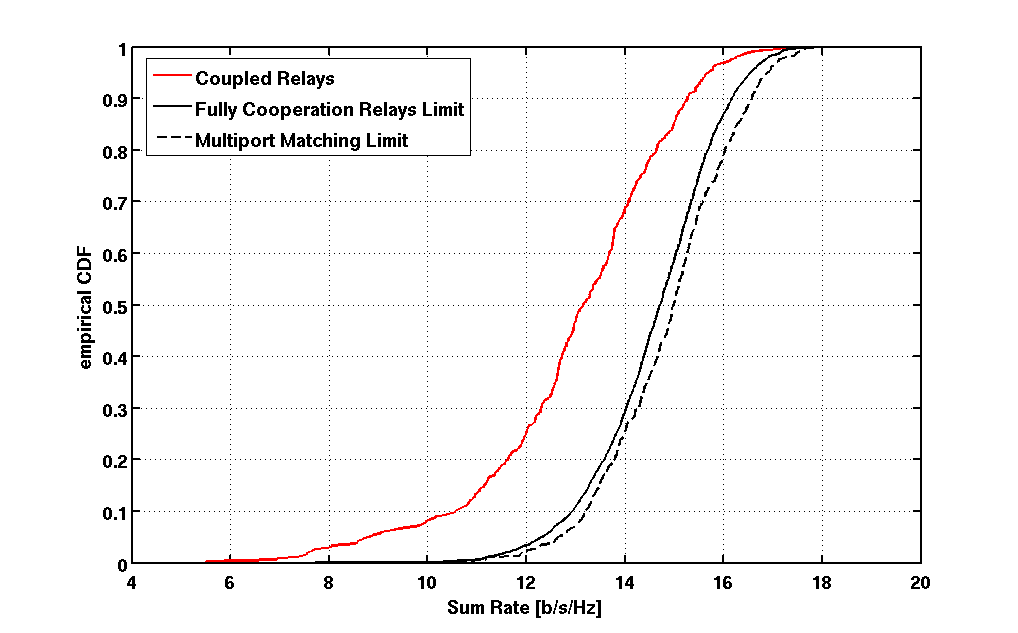
\includegraphics[width=0.9\linewidth]{images/Limitcomparison.png}
\caption{Comparison of the full cooperation relay rates, the multiport matching rate and optimized coupled relays rate.}
\label{fig:limcomparison}
\end{figure}

In Figure~\ref{fig:limcomparison} this limit is shown by the black dashed line.
It is a little bit higher than the fully cooperation relays performance.

\section{Relay Placing}
\label{sec:relay_placing}

Before analyzing the solver with different settings, the placing of the relays around a receiver is discussed a bit more in detail.
Figure~\ref{fig:cloud} shows, by which criteria, the relays were placed.
The red solid line denotes a zone around the receiver, in which no relays must be placed.
The red dashed line shows the maximum distance at which the relays may be placed away from the receiver. 
Within those two lines, the relays are thrown uniformly distributed.
The blue line around the relay at the right bottom denotes a zone in which no other relay may be placed, i.e. the minimum distance between each relay.
If there is a violation by the relay distances, all the relays are thrown again.
\begin{figure}[h]
\centering
  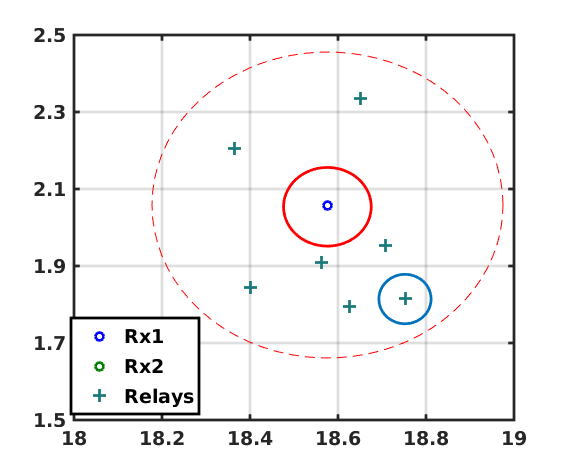
\includegraphics[width=0.9\linewidth]{images/cloud.png}
\caption{Placing the relays around a receiver uniformly distributed on a disk.}
\label{fig:cloud}
\end{figure}

The minimum receiver distance and the minimum relay distance might differ, however, if not specially mentioned, they are assumed to be both $0.1\lambda$.



\section{Relays to Zeroforce Interference}
\label{sec:interf_fix}

\subsection{One Interferer}
\label{sec:1interf}
\begin{figure}[h]
\centering
  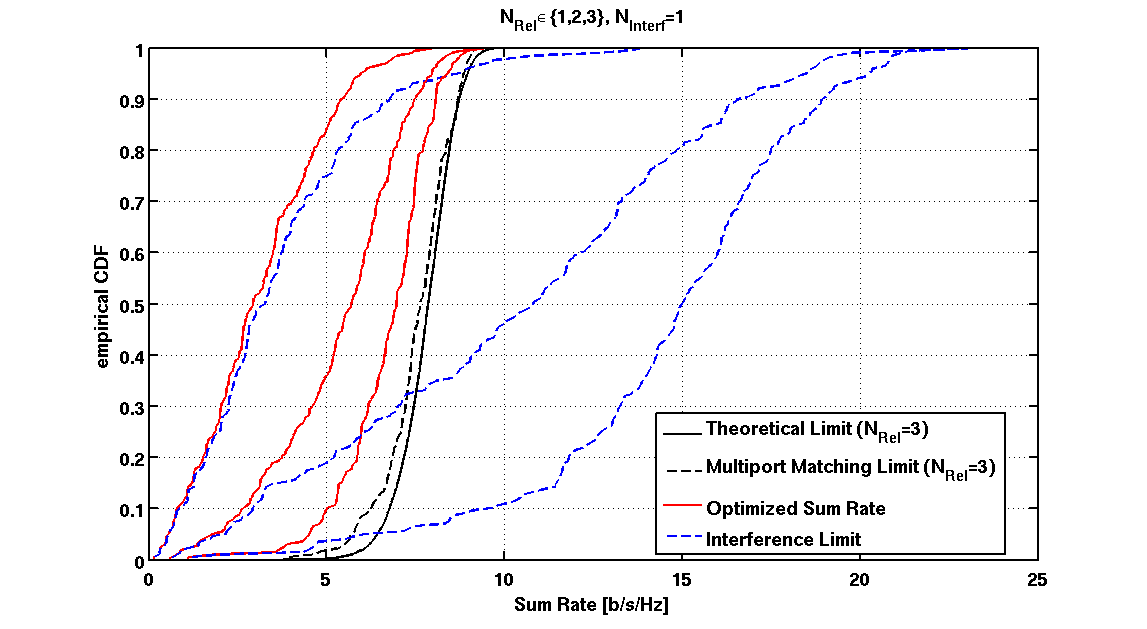
\includegraphics[width=0.9\linewidth]{images/Relcomparison_1interferer.png}
\caption{Sum rates for one interferer and one receiver with  $N_\text{Rel}\in\{1,2,3\}$.}
\label{fig:relcomp_1}
\end{figure}

\subsection{Two Interferer}
\label{sec:2interf}
\begin{figure}[h]
\centering
  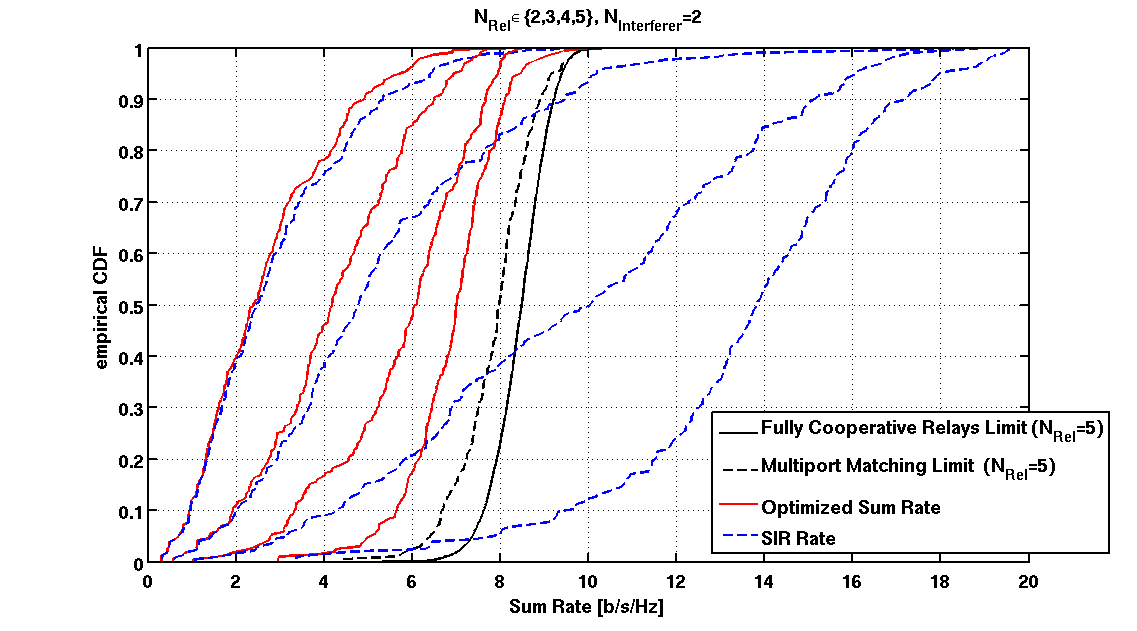
\includegraphics[width=0.9\linewidth]{images/Relcomparison_2interferer.png}
\caption{Sum rates for two interferer and one receiver with  $N_\text{Rel}\in\{2,3,4,5\}$.}
\label{fig:relcomp_2}
\end{figure}

\subsection{Three Interferer}
\label{sec:3interf}
\begin{figure}[h]
\centering
  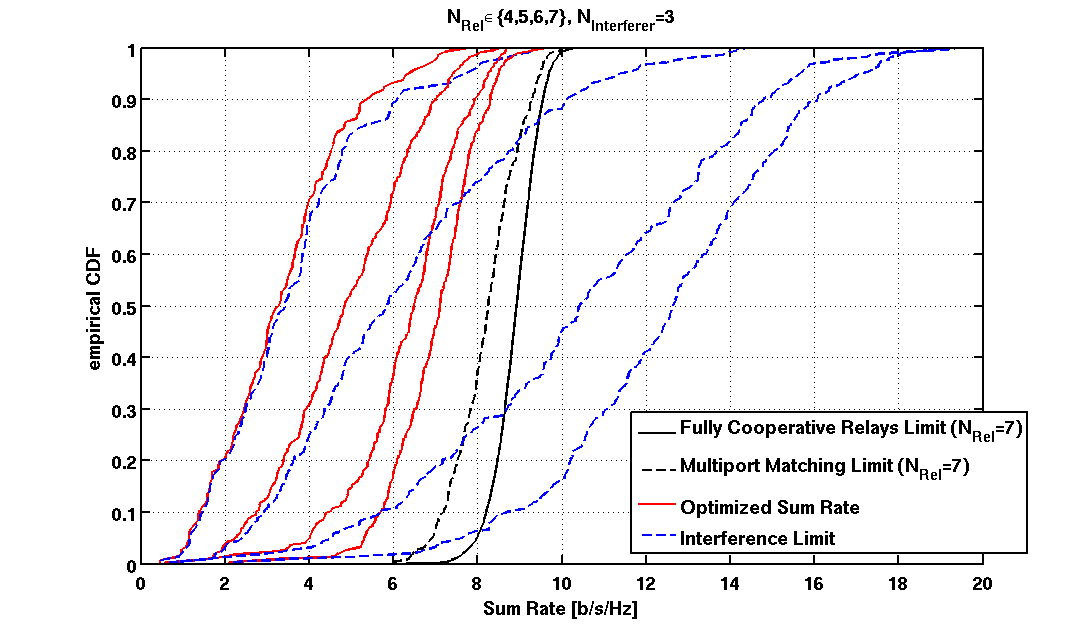
\includegraphics[width=0.9\linewidth]{images/Relcomparison_3interferer.png}
\caption{Sum rates for three interferer and one receiver with $N_\text{Rel}\in\{4,5,6,7\}$.}
\label{fig:relcomp_3}
\end{figure}


\section{Relay versus Rx Antenna Zeroforcing}
\label{sec:rel_place}


\section{Low SNR performance}
\label{sec:low_snr}

